\documentclass[10pt,twocolumn]{article}
\usepackage[utf8]{inputenc}
\usepackage[margin=0.75in]{geometry}
\usepackage{hyperref}
\usepackage{graphicx}
\usepackage{enumitem}
\usepackage{titlesec}
\usepackage{booktabs}
\usepackage{array}
\usepackage{float}
\usepackage{xcolor}
\usepackage{listings}

% Listings style for short code excerpts
\definecolor{codegray}{rgb}{0.4,0.4,0.4}
\definecolor{codeblue}{rgb}{0.1,0.1,0.55}
\lstset{
  basicstyle=\ttfamily\scriptsize,
  keywordstyle=\color{codeblue}\bfseries,
  commentstyle=\color{codegray}\itshape,
  breaklines=true,
  breakatwhitespace=true,
  columns=fullflexible,
  showstringspaces=false,
  extendedchars=true,
  frame=single,
  framesep=3pt,
  xleftmargin=2pt,
  aboveskip=4pt,
  belowskip=4pt,
  literate={º}{{\textordmasculine}}1 {ã}{{\~a}}1 {á}{{\'a}}1
           {é}{{\'e}}1 {í}{{\'i}}1 {ó}{{\'o}}1 {ç}{{\c c}}1
}

% Compact section formatting
\titlespacing*{\section}{0pt}{8pt plus 2pt minus 2pt}{4pt plus 2pt minus 2pt}
\titlespacing*{\subsection}{0pt}{6pt plus 2pt minus 2pt}{3pt plus 2pt minus 2pt}
\titlespacing*{\subsubsection}{0pt}{4pt plus 2pt minus 2pt}{2pt plus 2pt minus 2pt}

% Compact list formatting
\setlist{noitemsep, topsep=2pt, leftmargin=*}

% Title formatting
\title{\textbf{UbiGuard - Ubiquitous Security and Monitoring System (IoT and Mobile Systems 2025/26)}}
\author{
Afonso Simões, 73204
\and
Francisca Inácio, 73986
\and
Nasha Bagasse, 60913
}
\date{May 29, 2026}

\begin{document}
\maketitle

\section{Introduction}
Home security remains one of the most pressing concerns for residential property owners. This project consists of a complete IoT solution for residential security and automation. The system integrates a mobile application, a cloud-based backend, a web-based surveillance camera node, and one or more ubiquitous sensing devices built around an ESP32 microcontroller (the Gateway), forming an N-to-M architecture in which multiple users can monitor and control multiple secured zones.

\subsection{Context and Problems}
Burglaries affect millions of households each year, particularly in urban and suburban areas where properties may remain unoccupied for extended periods during working hours. Even though smart-home adoption has been growing, many affordable systems do not handle network failures gracefully, leaving homes effectively unprotected when connectivity drops: alarms that sound locally but fail to notify the homeowner remotely, or systems that cannot distinguish between a resident arriving home and an unauthorized entry.

The geographic scale of this project targets a single residential unit, such as a house or an apartment. The architecture, however, is designed so that a single user can manage several alarms (e.g., a main home and a vacation house) and a single alarm can be shared with several users (family members, occasional guests, etc.).

\subsection{Users and Roles}
The mobile application provides a carefully designed graphical interface and allows on-demand commands like arming/disarming remotely, checking the current temperature, inspecting the live status of the sensors, watching the live camera feed, and reviewing the full event log. The system is relevant because it transforms the smartphone users already carry into a context-aware security hub.

The system supports two account types at registration time --- \textbf{Installer} and \textbf{User} --- and a per-alarm permission model that further distinguishes \textbf{Owner}, \textbf{Child}, and \textbf{Guest} roles.

\subsubsection{User Profile Management}
\begin{itemize}
    \item \textbf{Installer Profile:} Used by the technician that physically installs the device. The installer can browse every alarm in the database, inspect its sensors, read its event logs, and perform the initial activation (binding a physical device to an Owner email and saving the home GPS coordinates). The installer does \emph{not} have access to the live camera feed or to the day-to-day arm/disarm controls.
    \item \textbf{Owner Profile:} The primary administrator of an alarm. The owner has full control: arm/disarm, change the alarm PIN, view the camera feed, read the event history, and grant or revoke access to other users (Child or Guest).
    \item \textbf{Child / Guest Profiles:} Both have the same baseline capabilities (arm, disarm, view the live camera feed, watch the event log) but cannot change the PIN, delete the alarm, or manage access. The Guest role is time-bounded: the Owner picks an expiry date/time when granting access, and once it elapses the App automatically removes the entry from the alarm and from the user's dashboard. The Child role has no expiry.
\end{itemize}

\subsection{Main Objectives}
The main objectives of this project are to design and implement a complete multi-component IoT architecture connecting mobile clients, a cloud backend, and sensing nodes through appropriate communication protocols; to provide context-aware security behaviours that respond both to sensor data and to occupant presence; to allow authorized users to monitor and control the system remotely; to enforce a role-based access model with distinct Installer, Owner, Child, and Guest profiles supporting time-bound temporary access; and to tolerate communication drops and power failures without losing observability.

\section{General Overview}

\subsection{Architecture}
UbiGuard is designed with an architecture that supports N-to-M relationships between clients (Mobile App instances), the cloud backend (Firebase), and controllers (ESP32 gateways).

To avoid overloading any central component with individual communication from dozens of sensors, the architecture relies on a Local Gateway installed in the residence. This microcontroller communicates locally with all the sensors and actuators wired to it, runs the time-critical logic on-device, and synchronizes state with Firebase (acting as the central cloud backend) over a secure connection. Firebase was chosen because it provides real-time database synchronization, anonymous and email/password authentication out of the box, and an SDK that the Android client can use directly, removing the need to host and maintain a dedicated server for the prototype.

Communication relies on the \textbf{Firebase Realtime Database} as a shared synchronization layer rather than a traditional message broker. The ESP32 gateway maintains a persistent, authenticated streaming connection to the database: it pushes sensor readings, state changes, and event logs, and keeps a stream listener open on its own subtree so that commands from the App (arm, disarm, PIN change) are pushed to the device in real time. The mobile App uses the Firebase Android SDK to listen to the same subtree, so updates from the gateway are reflected almost instantly on the dashboard, and writes commands directly to the database for the gateway to pick up. This streaming-listener model gives the low latency expected of an alarm system without the need to deploy or operate a separate message broker.

Asynchronous alerts on the user's phone (intrusion fired, status changed, PIN changed, alarm went offline, ``you forgot to arm'') are produced by a long-lived Android \textbf{foreground service} (\texttt{AlarmMonitorService}). The service holds Firebase listeners on the alarms the user has access to and posts Android system notifications even when the App is in the background. The system therefore does \emph{not} depend on Firebase Cloud Messaging or on Cloud Functions: all reactive logic lives either on the ESP32, on the mobile device, or in the database listeners themselves.

\subsection{Ubiquitous Integration with Mobile Sensors}
The application uses the smartphone's native sensors to create context-aware behaviours:
\begin{itemize}
    \item \textbf{Wi-Fi detection (arrival home):} When the user's phone (re)connects to the same Wi-Fi SSID that the alarm is connected to, the App writes a disarm command for that alarm to Firebase, so the system is unlocked by the time the user reaches the door.
    \item \textbf{Wi-Fi loss + GPS (leaving home):} When the phone loses the home Wi-Fi network, the foreground service enters ``Radar Mode'' and starts polling the GPS once per minute. If the user moves more than a configurable distance (1000\,m by default) from the saved home coordinates and the alarm is still disarmed, the App posts a high-priority notification (``Left home?'') with an inline \textbf{Arm Now} action that arms the alarm without opening the App.
    \item \textbf{Home location capture:} The home coordinates are not hardcoded. They are captured automatically from the installer's smartphone GPS at the moment the alarm is activated on-site and stored in the alarm record on Firebase.
\end{itemize}

\subsection{IoT Devices, Sensors and Actuators}
The ubiquitous layer is built around a single ESP32 microcontroller, chosen for its built-in Wi-Fi connectivity, low power consumption, and processing capacity sufficient to run local automation logic during offline operation. The gateway aggregates the data from all attached sensors, executes the immediate response logic locally, and synchronizes state with the cloud.

The local node uses a diverse set of devices, fulfilling the project requirement of at least two distinct sensor types and two distinct actuator types.

\subsubsection{Sensors}
\begin{itemize}
    \item \textbf{Magnetic Contact Sensor (MC-38):} Detects the opening of perimeter doors/windows.
    \item \textbf{PIR Motion Sensor (HC-SR501):} Detects volumetric presence indoors.
    \item \textbf{Temperature and Humidity Sensor (DHT11):} Continuous monitoring of the indoor climate, used for the fire-detection rule.
    \item \textbf{Membrane Keypad (4x4):} Physical interface for entering local PIN codes (arm, disarm, change PIN, silence fire alarm).
\end{itemize}

\subsubsection{Actuators}
\begin{itemize}
    \item \textbf{Visual Signaling Module (LEDs):} Green LED (system disarmed) and Red LED (system armed).
    \item \textbf{OLED Display (SSD1306 0.96" I2C):} Main visual interface that shows the current time and temperature, the system status (``ARMADO'', ``DESARMADO''), and special states (``DISPARADO!'' on intrusion, ``INCÊNDIO!'' on fire, ``NOVO PIN?'' during PIN change, ``Aguardando App...'' during initial pairing).
    \item \textbf{Active Buzzer:} High-intensity local audio alert, also used as feedback for keypad input.
    \item \textbf{Ubiquitous Surveillance Camera (Web Node):} The camera is not bound to a specific device. It is a WebRTC-based web page (\texttt{camera.html}) that can be opened on any spare device with a camera (smartphone, tablet, laptop) placed in the monitored space. The page listens to Firebase for an alarm trigger and a viewer request, and then negotiates a peer-to-peer WebRTC stream (using STUN/TURN servers) with the App.
\end{itemize}

\subsection{System Functionalities from the End User's Perspective}
Upon arriving home, the phone connects to the home Wi-Fi and the App automatically disarms the alarm, deactivating the siren standby and updating the local OLED to reflect the new state. Alternatively, a user standing at the door can disarm the system by typing the PIN on the membrane keypad, without reaching for the phone at all. When the user leaves the residence and forgets to arm the system, the App detects the Wi-Fi loss + GPS displacement combination and offers a one-tap arming action through a notification.

\subsubsection{Logic and Automatic Behaviors}
The system does not act in isolation; it presents automatic behaviours that depend on the combination of multiple inputs.
\begin{itemize}
    \item \textbf{Visual State Management:} When the system is armed (via the App, the keypad, or the local emergency Wi-Fi API), the gateway immediately updates the local interface: the Green LED turns off, the Red LED turns on, and the OLED switches the status line to ``ARMADO''. The reverse happens on disarm.
    \item \textbf{Intrusion Action:} While the alarm is armed, the gateway triggers immediately when the door magnetic contact reports ``open'' \emph{and} the PIR reports motion at the same time. The buzzer goes off continuously, the OLED switches to ``DISPARADO!'', and the \texttt{isFired} flag is written to Firebase. The App, observing that flag, posts a maximum-priority notification on the phone whose tap opens the live camera view.
    \item \textbf{Emergency Escalation through the Camera:} Tapping the intrusion notification opens the in-App viewer. The viewer writes \texttt{streamRequested = true} to Firebase, which wakes the camera node; the camera page acquires the local media stream and negotiates a WebRTC peer connection with the viewer. Closing the viewer tears down the connection.
    \item \textbf{Environmental Monitoring:} The DHT11 sensor is polled every two seconds. If the temperature rises above 60\,$^{\circ}$C, regardless of the alarm's armed/disarmed state, the system raises a fire alert: the OLED switches to ``INCÊNDIO!'', the buzzer sounds at a distinct high-pitched tone, and \texttt{isFired} is written to Firebase so the App posts a critical notification. The fire alarm can be silenced manually with \texttt{PIN + A} on the keypad and is automatically rearmed once the temperature drops back below 50\,$^{\circ}$C.
\end{itemize}

Members of the household with Child or Guest access can arm and disarm the alarm via the App with their own account (the keypad PIN is shared across the device), while Guest profiles allow temporary visitors the same App-level access for a time window defined by the Owner.

\subsubsection{Fault Tolerance and Communication Drops}
A security system must be resilient. UbiGuard addresses three categories of failure.

\textbf{Internet loss at the gateway.} The reactive logic lives on the ESP32, so the keypad PIN, the intrusion rule, and the fire rule keep working without internet. While offline, the gateway buffers up to 50 log entries in memory; when the connection comes back, those logs and the current snapshot of the state are pushed to Firebase in a single sync pass.

\textbf{Internet loss as a feature: the Emergency AP.} When the ESP32 detects that the home Wi-Fi is down, it brings up a soft access point named \texttt{UbiGuard\_Emergencia} protected with a password derived from the current PIN, and exposes a small HTTP REST API on \texttt{192.168.4.1} (\texttt{/status}, \texttt{/armar}, \texttt{/desarmar}). The Android App detects this SSID and switches to direct local HTTP communication for that alarm, so the Owner can still arm or disarm and read sensor state even with the home internet down.

\textbf{Power outage or sabotage.} The ESP32 publishes a \texttt{heartbeat} value to Firebase every 30 seconds. The App's foreground service starts a 65-second watchdog every time it receives a heartbeat; if the watchdog fires (no heartbeat in 65\,s), the App posts an ``Alarm Offline'' warning. When heartbeats resume, an ``Alarm Online'' notification is posted.

\subsection{Component Interaction}
All components interact through the Firebase backend, which mediates every exchange. The ESP32 writes sensor readings, state changes, and event logs to its node in the Realtime Database, and keeps a streaming listener open on the same node to receive instructions (arm/disarm, PIN change, camera-trigger flags) as soon as they are written by another client.

The mobile App writes commands and configuration directly to the database through the Firebase SDK and observes the relevant paths to receive real-time updates. Time-critical alerts are surfaced as Android system notifications by the \texttt{AlarmMonitorService} foreground service, which holds the database listeners on the user's behalf even while the App is not in the foreground.

The GPS and Wi-Fi sensors on the user's phone feed data to the App locally; the App evaluates them and writes arming suggestions or automatic disarming commands to the backend when the user leaves or arrives at the residence.

The surveillance camera node (the \texttt{camera.html} page) authenticates anonymously to Firebase, listens to the alarm's \texttt{isFired} and \texttt{webrtc/streamRequested} flags, and when both are true negotiates a WebRTC peer connection with the App's in-App viewer using Firebase paths as the signalling channel.

In summary, the Firebase backend mediates all interactions: the mobile App, the ESP32 gateway, and the camera node do not communicate directly with one another (except during the WebRTC media leg itself, which is peer-to-peer once signalling is done), which keeps the architecture clean, scalable, and secure.

\subsection{Demonstration Prototype}
For the course prototype, the following components are implemented to demonstrate the full architecture at a reduced scale:
\begin{itemize}
    \item \textbf{1 Android mobile application} --- fully functional, supporting Installer, Owner, Child, and Guest roles with Wi-Fi-based automatic disarming, Wi-Fi-loss + GPS-based ``forgot to arm'' notifications, real-time push notifications, on-demand arm/disarm and PIN-change commands, an event history, and an in-App WebRTC camera viewer.
    \item \textbf{1 web-based surveillance camera node} --- a static HTML page (\texttt{camera.html}) running on any spare device with a camera placed in the monitored room, capable of receiving an activation command from the backend and streaming live video to the App via WebRTC.
    \item \textbf{Firebase Backend} --- the Realtime Database is used as the synchronization layer and Firebase Authentication is used for both anonymous device identities (gateway, camera) and email/password user accounts. The prototype intentionally does not deploy Cloud Functions: every reactive rule runs either on the ESP32 or on the Android device, which keeps the cloud footprint minimal.
    \item \textbf{1 ESP32 gateway node} --- simulates a full entry-point security station, equipped with the magnetic contact sensor (MC-38), the PIR motion sensor (HC-SR501), the DHT11 sensor, the 4x4 membrane keypad, the OLED display, the LED pair, and the active buzzer. It also implements the captive portal for Wi-Fi pairing (via WiFiManager), the offline log buffer, the emergency Wi-Fi access point and its REST API, and the heartbeat.
\end{itemize}

\section{System Architecture}
UbiGuard is organised in three tiers --- an edge tier, a cloud tier, and a client tier --- that never address one another directly except during the WebRTC media leg. Everything else passes through the cloud, which keeps the design loosely coupled and lets components join or leave without reconfiguring the others.

\subsection{Components}
\textbf{Edge tier.} The ESP32 gateway is the brain of the residence. It reads the MC-38 magnetic contact, the HC-SR501 PIR, and the DHT11 over GPIO, drives the OLED (I2C), the two LEDs and the active buzzer, and scans the 4x4 keypad. It holds all the time-critical logic so that the alarm keeps working even with no internet. The surveillance camera is a second, optional edge component: a static web page (\texttt{camera.html}) that runs on any spare device with a camera and only turns the lens on when an intrusion is in progress and a viewer asks for the stream.

\textbf{Cloud tier.} Firebase provides two services. \emph{Authentication} issues anonymous identities to the gateway and the camera page and email/password accounts to the human users. The \emph{Realtime Database} (RTDB) is the single point of synchronisation: every state change, command, log entry, and WebRTC signalling message is a write to a well-known path, and every component reacts by listening to the paths it cares about. No Cloud Functions are deployed; the database is used purely as a shared, observable state tree.

\textbf{Client tier.} The Android application is the control panel. Beyond its screens, it runs a foreground service (\texttt{AlarmMonitorService}) that keeps the Firebase listeners and the phone's sensors alive while the app is backgrounded.

\subsection{Data Model}
The database is rooted at two collections. Each alarm lives under \texttt{/alarms/\{alarmId\}} and holds its \texttt{status} (\texttt{Armado}/\texttt{Desarmado}), the shared \texttt{pin}, the \texttt{isFired} flag, the \texttt{activated} flag set by the installer, the \texttt{ownerId}, a \texttt{heartbeat} counter, a \texttt{network} object (\texttt{ssid}, \texttt{lat}, \texttt{lng}), a \texttt{sensors} subtree with the last reading of each device, an append-only \texttt{logs} list, an \texttt{access\_list} of the users who may use the alarm, and a \texttt{webrtc} subtree used as the signalling channel. Each user lives under \texttt{/users/\{uid\}} with their profile (\texttt{name}, \texttt{email}, \texttt{address}, \texttt{account\_type}) and an \texttt{alarms} map listing the alarms they can access, together with the role metadata (\texttt{isChild}, \texttt{expiry}). The alarm identifier is derived deterministically from the ESP32 MAC address (\texttt{alarm\_<MAC>}), so it is stable across reboots and unique per device.

\subsection{Communication and Protocols}
Each link uses the protocol best suited to it:
\begin{itemize}
    \item \textbf{Gateway $\leftrightarrow$ Firebase.} The ESP32 uses the Firebase ESP Client library over TLS. It keeps a persistent RTDB \emph{stream} open on its own \texttt{/alarms/\{alarmId\}} subtree (a long-lived HTTPS server-sent-events connection), so commands written by the app --- arm, disarm, PIN change --- arrive within a fraction of a second. Outgoing readings, log pushes, and the heartbeat are written asynchronously on the same connection.
    \item \textbf{App $\leftrightarrow$ Firebase.} The app uses the Firebase Android SDK, which keeps a WebSocket to the RTDB. Value listeners on the relevant paths give the dashboard near-instant updates, and commands are plain writes.
    \item \textbf{Camera $\leftrightarrow$ Firebase.} The camera page uses the Firebase JavaScript SDK with anonymous auth and listens to \texttt{isFired} and \texttt{webrtc/streamRequested}.
    \item \textbf{App $\leftrightarrow$ Camera.} Once both flags are set, the two peers negotiate a WebRTC connection using the \texttt{webrtc} subtree (offer, answer, and ICE candidates) as the signalling channel and public STUN/TURN servers for NAT traversal. The video itself then flows peer-to-peer, never touching Firebase.
    \item \textbf{App $\leftrightarrow$ Gateway (emergency).} When the home internet is down the gateway raises a soft access point and exposes a small HTTP REST API on \texttt{192.168.4.1}; the app talks to it directly with plain \texttt{GET} requests.
    \item \textbf{Time.} On boot the gateway synchronises its clock over NTP so that log timestamps are meaningful.
\end{itemize}

The interactions are mostly event-driven, with a few periodic tasks: the heartbeat is written every 30\,s, the DHT11 is polled every 2\,s, the app's watchdog expires 65\,s after the last heartbeat, and the GPS is polled once a minute while the phone is in Radar Mode.

\section{Mobile Application}
The mobile application is a native Android app written in Kotlin and targeting modern Android (notification, background-location, and foreground-service permissions are requested at runtime). It is the only interface a regular user ever touches.

\subsection{Technologies}
The app builds on the Firebase Android SDK for both Authentication (email/password) and the Realtime Database, the Google Play Services \emph{Fused Location Provider} for GPS, and the Android \texttt{ConnectivityManager}/\texttt{WifiManager} for Wi-Fi state. The live camera viewer is a \texttt{WebView} that loads the hosted \texttt{viewer.html} page and grants it camera/microphone permissions so the WebRTC stack runs inside the page. Background work uses a started \emph{foreground service}, a \emph{broadcast receiver} for the notification action button, and Kotlin coroutines for the local HTTP calls in emergency mode. The UI is built from standard Activities, RecyclerViews and adapters, with a side drawer shared across screens through a \texttt{BaseActivity}.

\subsection{Functionalities and Screens}
The login and registration screens create accounts, which default to the \texttt{User} type; the \texttt{Installer} type is promoted manually in the database. After login, the dashboard branches on the account type. An \emph{installer} sees activation and association controls and can browse every alarm in the system, with text and armed/disarmed filters, drilling into each alarm's sensors and logs (Figure~\ref{fig:installer-storyboard}). A regular \emph{user} sees only the alarms they have access to, loaded by cross-referencing \texttt{/users/\{uid\}/alarms} with \texttt{/alarms}; expired guest entries are pruned on the spot when the list is rendered.

Opening an alarm shows its live status and a single arm/disarm button, the ``safe/fired'' emergency indicator, and a shortcut to the event log. The owner additionally sees the access-management block: a dialog to grant Child (permanent) or Guest (with a date/time picker for the expiry) access by e-mail, and the list of current grants, each removable with a confirmation dialog. PIN changes are a simple write to \texttt{/alarms/\{id\}/pin}. Every screen reflects database changes in real time through value listeners, so an action taken on the keypad or by another user appears immediately (Figure~\ref{fig:owner-storyboard}).

\subsection{Background Intelligence}
The \texttt{AlarmMonitorService} is what makes the app context-aware. It attaches listeners to each accessible alarm for \texttt{isFired} (max-priority intrusion/fire notification whose tap opens the camera viewer), \texttt{status} and \texttt{pin} (informative notifications, suppressing the first callback so the initial load is silent), and \texttt{heartbeat} (a 65\,s watchdog that posts ``offline''/``online'' notifications). It also registers a network callback: when the phone joins the same SSID the alarm is on, it auto-disarms; when it loses that SSID it enters Radar Mode, polling GPS once a minute and, if the user drifts past the configured distance while the alarm is still disarmed, posting the ``Left home?'' notification with an inline \textbf{Arm Now} action handled by \texttt{ArmAlarmReceiver}.

\subsection{Data Management and Server-side Dependencies}
The app keeps almost no local state; the RTDB is the source of truth and the SDK's listeners drive the UI. The only client-side logic that mutates shared state autonomously is the expiry pruning of guest access and the automatic disarm/arm suggestions. The single server-side dependency is Firebase (Auth + RTDB); there is no custom backend. The one exception to the cloud-mediated rule is emergency mode: when the phone is connected to the \texttt{UbiGuard\_Emergencia} access point, the alarm-details screen and the arm receiver bypass Firebase entirely and issue HTTP requests to the gateway, polling \texttt{/status} every two seconds to keep the UI live.

\begin{figure*}[t]
    \centering
    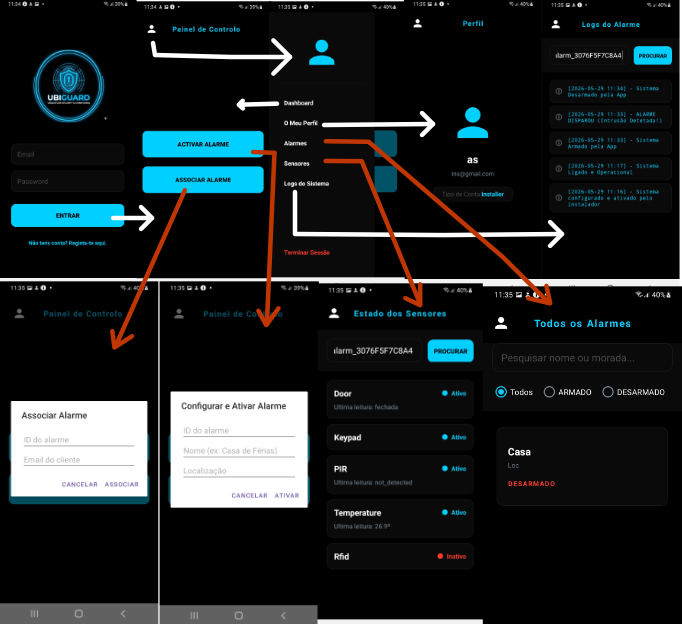
\includegraphics[width=\textwidth]{images/installer_storyboard.jpg}
    \caption{Installer storyboard: from login the installer reaches the control panel, where they can activate a new alarm or associate an existing one to an owner, browse the system-wide alarm list with text and armed/disarmed filters, and drill into each alarm's sensor state and event logs.}
    \label{fig:installer-storyboard}
\end{figure*}

\begin{figure*}[t]
    \centering
    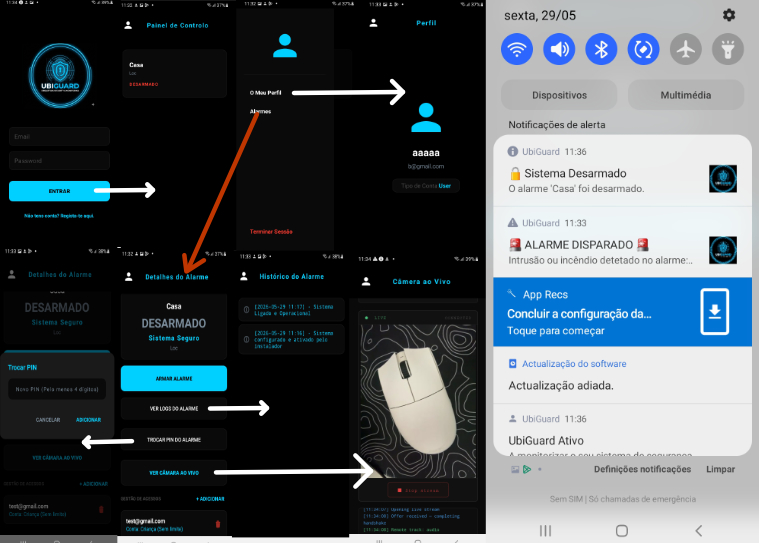
\includegraphics[width=\textwidth]{images/owner_storyboard.jpg}
    \caption{Owner storyboard: after login the owner sees only their accessible alarms, opens an alarm to arm/disarm it, change the PIN, review the event history, and open the live WebRTC camera viewer, while the foreground service surfaces real-time alerts (armed/disarmed, intrusion fired, configuration reminders) as Android system notifications.}
    \label{fig:owner-storyboard}
\end{figure*}

\section{Sensing and Reacting}
All sensors and actuators are real, off-the-shelf components wired to the ESP32; nothing in the local node is simulated. The only ``virtual'' device is the surveillance camera, which is realised as a web page running on a spare phone or laptop rather than a dedicated camera board, precisely because the project treats the camera as a ubiquitous, device-independent node.

\begin{figure*}[t]
    \centering
    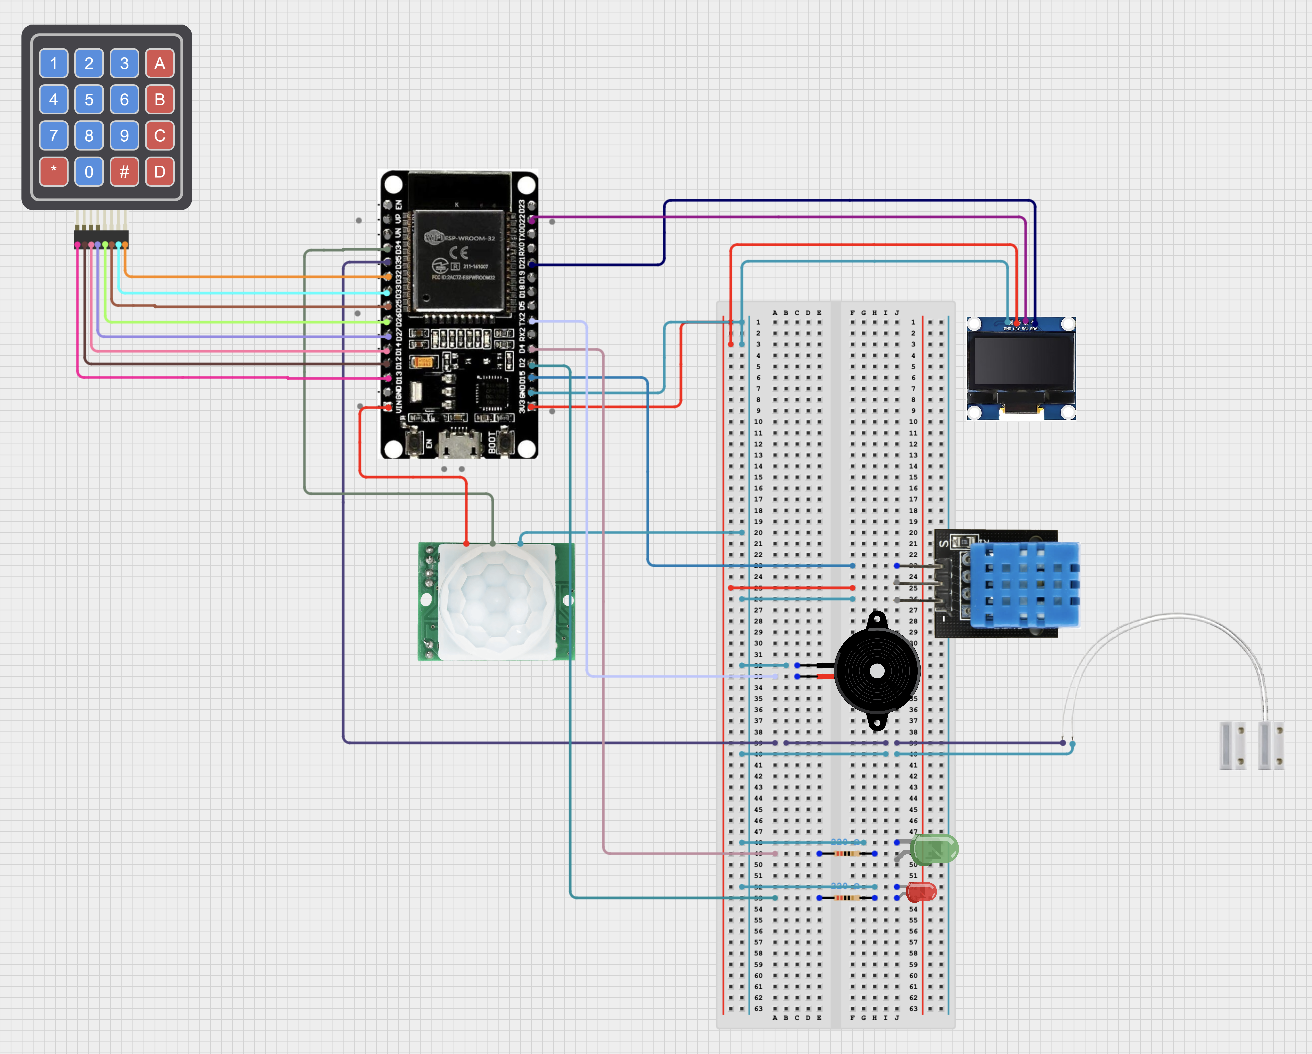
\includegraphics[width=\textwidth]{images/schematic.png}
    \caption{Wiring of the UbiGuard gateway: the ESP32 connects the 4x4 keypad, the PIR motion sensor, the MC-38 magnetic contact, the DHT11, the SSD1306 OLED, the active buzzer, and the green/red status LEDs.}
    \label{fig:schematic}
\end{figure*}

Figure~\ref{fig:schematic} shows the wiring. The door contact is read with the internal pull-up (\texttt{INPUT\_PULLUP}) so a closed door reads \texttt{LOW} and an open door reads \texttt{HIGH}; the PIR is a plain digital input on a pin without internal pull-ups (GPIO\,34); the DHT11 is read over its one-wire protocol; the OLED shares the I2C bus; and the keypad occupies eight GPIOs as a row/column matrix.

\subsection{Reading and Reflecting the Sensors}
The main loop is non-blocking. The door and PIR are read every iteration and, on a state change, the new reading is mirrored to the database and added to the log. The DHT11 is sampled on a 2\,s timer, and a reading is only published when it actually moves (a 0.1$^{\circ}$C dead-band) to avoid flooding the database:

\begin{lstlisting}[language=C++]
if (millis() - lastDhtRead > 2000) {
  lastDhtRead = millis();
  float temp = dht.readTemperature();
  if (!isnan(temp) && abs(temp-lastTemp) >= 0.1) {
    lastTemp = temp;
    Firebase.RTDB.setStringAsync(&fbdo,
      ".../sensors/Temperature/last_read",
      String(temp,1) + "º");
  }
  // ... fire rule below ...
}
\end{lstlisting}

\subsection{Autonomic Reactions}
The ``smart'' behaviour comes from combining several signals locally so the system reacts in milliseconds, with no round-trip to the cloud.

\textbf{Intrusion.} The alarm fires only when it is armed \emph{and} the door is open \emph{and} the PIR sees motion at the same time --- the conjunction sharply reduces false positives from, e.g., a curtain moving near the PIR. Firing latches the buzzer, repaints the OLED, and raises \texttt{isFired} for the app and camera to observe:

\begin{lstlisting}[language=C++]
if (armed && currentPirState == HIGH
    && currentDoorState == HIGH
    && !alarmTriggered) {
  alarmTriggered = true;
  if (!fireTriggered) tone(BUZZER_PIN, 1000);
  addLog("ALARME DISPAROU (Intrusao Detetada!)");
  Firebase.RTDB.setBoolAsync(&fbdo,
    ".../isFired", true);
  updateDisplay();
}
\end{lstlisting}

\textbf{Fire.} Independently of the armed state, a temperature above 60$^{\circ}$C raises a distinct high-pitched alarm and sets \texttt{isFired}; it auto-rearms once the temperature falls back below 50$^{\circ}$C (the hysteresis gap stops the alarm from chattering around the threshold). It can also be silenced on the spot with \texttt{PIN + A}.

\textbf{Local control and feedback.} The keypad handler interprets \texttt{PIN + \#} as an arm/disarm toggle, \texttt{PIN + B} as the start of a PIN change, and \texttt{PIN + A} as a fire-silence, giving audible feedback on every keypress and writing the resulting state back to Firebase. The two LEDs and the OLED are updated synchronously through \texttt{updateLeds()} and \texttt{updateDisplay()} so the physical panel and the app never disagree.

\subsection{Reacting on the Phone}
The phone closes two context-aware loops the gateway cannot see. When the foreground service detects the phone has joined the alarm's SSID, it disarms automatically; the comparison is between the phone's current SSID and the one the gateway stored under \texttt{network/ssid}:

\begin{lstlisting}
if (alarmSSID != null && alarmSSID == phoneSSID) {
    stopRadarMode()
    database.child("alarms").child(alarmId)
        .child("status").setValue("Desarmado")
    database.child("alarms").child(alarmId)
        .child("isFired").setValue(false)
}
\end{lstlisting}

Conversely, on Wi-Fi loss the service polls the Fused Location Provider and, using \texttt{Location.distanceBetween} against the home coordinates captured at install time, decides whether the user has really left and still forgot to arm before nudging them. This pair of rules is what turns a phone the user already carries into the presence sensor of the system.

\section{Experiments}
We validated the system end-to-end on real hardware (a physical ESP32 with all sensors wired as in Figure~\ref{fig:schematic}) and a physical Android phone, since emulators do not reproduce background Wi-Fi and GPS behaviour reliably. Each experiment below states its purpose, the assumptions it relies on, and what we did. Where a threshold made a test impractical (walking a kilometre, heating a sensor to 60$^{\circ}$C), we temporarily lowered it in code, which does not change the logic under test.

\subsection{Installer Setup and Location Capture}
\emph{Purpose:} confirm that a fresh device can be paired to a network and an owner without hardcoding anything. \emph{Assumptions:} the installer is physically at the property with GPS enabled. \emph{Test:} we powered a blank ESP32, joined its captive portal (\texttt{UbiGuard\_XXXX}), selected the home router, set the keypad PIN, and from an installer account activated the alarm by its on-screen ID and associated it to an owner e-mail. We then inspected the database and confirmed the alarm record carried the correct SSID and the installer's latitude/longitude, captured automatically at activation.

\subsection{Geofencing ``Forgot to Arm''}
\emph{Purpose:} verify the Wi-Fi-loss + GPS rule. \emph{Assumptions:} background-location permission granted; the alarm is disarmed. \emph{Test:} with the threshold lowered to 1\,m, we disconnected the phone from the home Wi-Fi, walked a few steps, and waited for the GPS poll. The ``Left home?'' notification appeared, and tapping \textbf{Arm Now} armed the alarm and switched the OLED to \texttt{ARMADO} within seconds --- without opening the app.

\subsection{Automatic Disarm on Arrival}
\emph{Purpose:} verify the inverse rule. \emph{Test:} starting from an armed alarm with the phone off the home network, we reconnected the phone to the alarm's SSID and observed the alarm disarm automatically and the LEDs/OLED follow.

\subsection{Physical Intrusion}
\emph{Purpose:} confirm the armed/door/PIR conjunction. \emph{Test:} with the system armed we separated the magnet and triggered the PIR; the buzzer latched, the OLED showed \texttt{DISPARADO!}, and the phone received a maximum-priority alert. Triggering only one of the two sensors did \emph{not} fire the alarm, confirming the conjunction. Entering \texttt{PIN + \#} on the keypad and pressing disarm in the app both cleared it.

\subsection{Fire Detection and Silencing}
\emph{Purpose:} confirm the temperature rule works regardless of armed state and self-rearms. \emph{Test:} with the thresholds temporarily lowered, we warmed the DHT11 with breath until the alarm fired with its distinct tone and \texttt{INCÊNDIO!} on the OLED; \texttt{PIN + A} silenced it, and letting the sensor cool re-armed the fire logic automatically.

\subsection{Role-Based Access Control}
\emph{Purpose:} validate the permission model and guest expiry. \emph{Test:} an owner granted a second account Child and Guest access by e-mail; logging in as that account, the alarm appeared on its dashboard with only arm/disarm controls --- no PIN change, deletion, or access management. For a Guest with a near expiry, the entry was removed from both the alarm and the dashboard once the deadline passed.

\subsection{Fault Tolerance}
\emph{Purpose:} confirm the system survives loss of internet and power. \emph{Tests:} (i) with the router off, the keypad, intrusion and fire rules kept working, and on reconnection the buffered logs and current state synced up in one pass; (ii) connected to the \texttt{UbiGuard\_Emergencia} access point, the app armed/disarmed and read sensor state over the local REST API; (iii) cutting power to the gateway produced an ``Alarm Offline'' notification after $\sim$65\,s, and restoring it produced ``Alarm Online''.

\subsection{Live Camera Escalation}
\emph{Purpose:} confirm the on-demand WebRTC pipeline. \emph{Test:} after an intrusion, tapping the notification opened the in-app viewer, which woke the camera page; the page acquired the local stream and a peer-to-peer connection was established through the Firebase signalling channel. Closing the viewer tore the connection down and cleared the signalling data, leaving the camera idle.

\section{Conclusions and Lessons Learned}
UbiGuard met the goals it set out with: a multi-component IoT system in which several users can monitor and control several alarms, with context-aware automation, a role-based access model, and graceful degradation when connectivity or power fails. Building it taught us as much about the gaps between a working prototype and a deployable product as about the technologies themselves.

\subsection{Towards a Real-World Deployment}
Several decisions that are reasonable for a course prototype would have to change in production. The most important is \textbf{security}. The Realtime Database runs with permissive rules so that any authenticated client can read and write any alarm; a real system needs per-path security rules tying writes to the alarm's owner and access list, the PIN should never be stored in clear text, and the TURN credentials and Firebase keys embedded in the camera page would have to be moved server-side and rotated. The emergency access point currently derives its password from the PIN and serves plain HTTP, which is acceptable as a last-resort local channel but should at least use a stronger key and authenticated requests.

\textbf{Reliability} is the other axis. A burglar can defeat the gateway by cutting power, so a real unit needs a battery backup and ideally a cellular fallback for notifications when the home internet is down --- today an attacker who kills both power and Wi-Fi only triggers an ``offline'' warning. Replacing the foreground-service-plus-listeners notification path with Firebase Cloud Messaging would also be more battery-friendly and more reliable across aggressive OEM background-killing policies, at the cost of introducing Cloud Functions. Finally, tamper detection (an enclosure switch), over-the-air firmware updates, and a proper commissioning flow would all be expected of a shipping product.

\subsection{Lessons Learned}
The clearest lesson was the value of \textbf{putting the time-critical logic at the edge}. Because the intrusion and fire rules live on the ESP32, the system stays useful with no internet, and the cloud becomes a synchronisation and notification layer rather than a dependency on the critical path. The flip side is that keeping the edge state and the cloud state consistent --- especially across reconnections --- required care, and the offline log buffer plus single-pass resync was the cleanest way we found to handle it.

We also learned how much of ``ubiquitous'' behaviour comes from \textbf{the phone rather than the dedicated hardware}. Wi-Fi presence and GPS displacement turned an ordinary smartphone into the system's occupancy sensor, but Android's tightening restrictions on background location and Wi-Fi SSID access made this the most fragile part of the project and the reason a physical device was indispensable for testing. Treating the camera as a device-independent web node, rather than buying a camera board, was another pragmatic win: WebRTC let us stream peer-to-peer with Firebase used only for signalling, and any spare phone became a camera. Getting the WebRTC handshake robust --- queuing ICE candidates until the remote description is set, and tearing the connection down cleanly --- was the subtlest engineering of the whole project, and a good reminder that the ``last mile'' of a real-time feature is where most of the effort hides.

\begin{thebibliography}{9}
\bibitem{bjs} \emph{Victimization During Household Burglary}, BJS, U.S. Department of Justice --- \url{https://bjs.ojp.gov/content/pub/pdf/vdhb.pdf}
\end{thebibliography}

\end{document}
